\documentclass[10pt, a4paper]{article}
\usepackage[T1]{fontenc}
\usepackage[utf8]{inputenc}
\usepackage[english]{babel}
\usepackage{tikz}
\usepackage{pgfplots}
\pgfplotsset{compat=1.10}
\usepackage{amsmath}
\usepackage{url, hyperref}


\renewcommand{\textfraction}{0.001}
\renewcommand{\topfraction}{0.999}   
\renewcommand{\bottomfraction}{0.999}


\setlength{\parindent}{0pt}
\begin{document}

\section{Einfache Tikz Befehle}
Tikz steht fuer: \textit{Tikz ist kein Zeichenprogramm}, also ein rekursives Akronym. Tikz erstellt uns Vektorgrafiken. Vektorgrafiken lassen sich beliebig skalieren.

Eine ausf"uhrlichere Einleitung in Tikz findet ihr hier: \url{http://cremeronline.com/LaTeX/minimaltikz.pdf}


\subsection{Draw-Befehl}
\begin{tikzpicture}
\draw (0,0) --(1,2);
\end{tikzpicture}

\subsection{Optionen}

Man kann sich zum Beispiel ein Hilfsgitter zeichnen lassen:

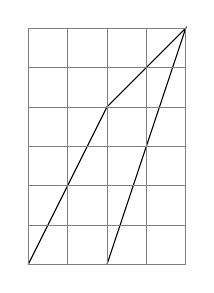
\begin{tikzpicture}
\draw (0,0) --(1,2) -- (2,3) -- (1,0);
\draw[help lines, step=0.5] (0,0) grid (2,3);
\end{tikzpicture}

\begin{figure}[h]
\centering
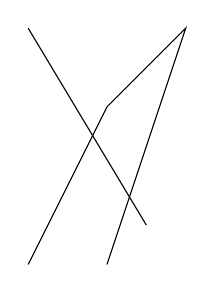
\begin{tikzpicture}
\draw (0,0) -- (1,2) -- (2,3) -- (1,0);
\draw (0,3) -- (1.5,0.5);
\end{tikzpicture}
\caption{Tikz-Bilder kann man auch in einer Float verwenden}
\end{figure}

\subsection{Vektoren/Pfeile}

\begin{tikzpicture}
\draw [<->] (0,2) -- (0,0) -- (3,0);
\draw [->] (0,0) -- (2,2);
\draw [<-] (0,1) -- (2,3);
\end{tikzpicture}

\subsection{"Andern der Linienbreite}


\begin{tikzpicture}
\draw [ultra thick] (0,1) -- (2,1);
\draw [thick] (0,0.5) -- (2,0.5);
\draw [thin] (0,0) -- (2,0);
\end{tikzpicture}

M"ogliche Befehle um die Linienbreite zu "andern:

\begin{itemize}
\item ultra thin
\item very thin
\item thin
\item semithick
\item thick
\item very thick
\item ultra thick
\end{itemize}

\section{Funktionen zeichnen mit Tikz}
\begin{center}
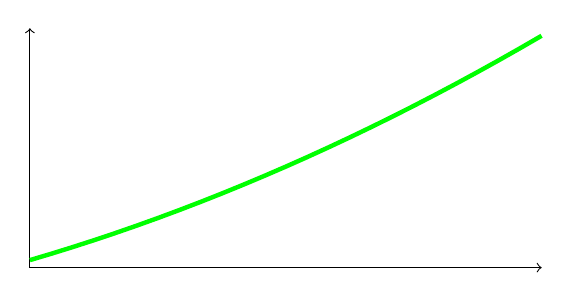
\begin{tikzpicture}[xscale=13,yscale=3.8] % Man kann die Zeichnung auch skalieren
\draw [<->] (0,0.8) -- (0,0) -- (0.5,0);
\draw[green, ultra thick, domain=0:0.5] plot (\x, {0.025+\x+\x*\x});
\end{tikzpicture}
\end{center}

\begin{figure}[h]
\centering
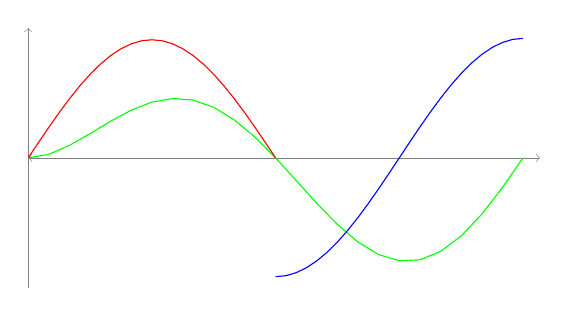
\begin{tikzpicture}[yscale=1.5] % Hier ist nur die y-Achse skaliert
\draw [help lines, <->] (0,0) -- (6.5,0);
\draw [help lines, ->] (0,-1.1) -- (0,1.1);
\draw [green,domain=0:2*pi] plot (\x, {(sin(\x r)* ln(\x+1))/2});
\draw [red,domain=0:pi] plot (\x, {sin(\x r)});
\draw [blue, domain=pi:2*pi] plot (\x, {cos(\x r)*exp(\x/exp(2*pi))});
\end{tikzpicture}
\caption{In Tikz kann man Winkel in Grad oder Radiant angeben. Will man es in Radiant angeben, muss man dies mit einen \texttt{r} so kennzeichnen.}
\end{figure}

  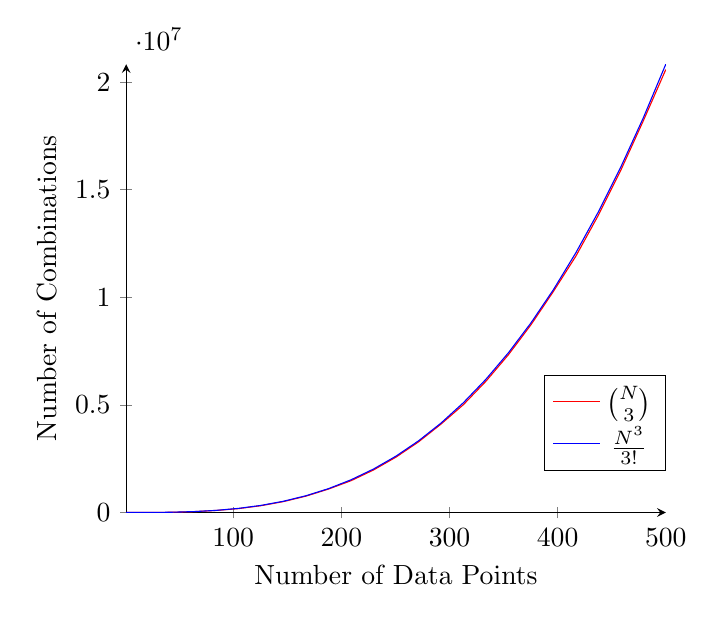
\begin{tikzpicture}
    \begin{axis}[
    axis lines = left,
    xlabel = Number of Data Points,
    ylabel = {Number of Combinations},
    legend style={at={(1,0.2)},anchor=east},
    ]
    \addplot [
    domain=1:500, 
    color=red,
    ]
    { factorial(x)/(factorial(x-3)*factorial(3))};
    \addplot [
    domain=1:500, 
    color=blue,
    ]
    { x^3/factorial(3)};
    \addlegendentry{$\binom{N}{3}$}
    \addlegendentry{$\frac{N^3}{3!}$}
    \end{axis}

  \end{tikzpicture}


\section{Verwendung von "`Nodes"'}
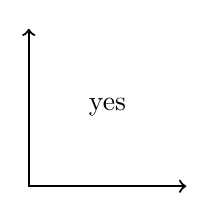
\begin{tikzpicture}
\draw [thick, <->] (0,2) -- (0,0) -- (2,0);
\node at (1,1) {yes};
\end{tikzpicture}

\vspace{5mm}

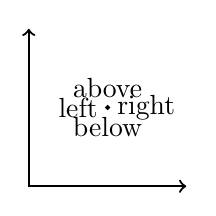
\begin{tikzpicture}
\draw [thick, <->] (0,2) -- (0,0) -- (2,0);
\draw[fill] (1,1) circle [radius=0.025];
\node [below] at (1,1) {below};
\node [above] at (1,1) {above};
\node [left] at (1,1) {left};
\node [right] at (1,1) {right};
\end{tikzpicture}

\section{Sich wiederholende Strukturen in Tikz}
\begin{tikzpicture}[yscale = 0.2]
\foreach \x in {1,2,...,6}{
\draw (\x,-0.5) -- (\x,1);
\draw (0, \x) -- (0.5,\x);
}
\end{tikzpicture}
\end{document}
